% ================================================================= STATE ==
\section{Task 1: state reconstruction}\label{sec:state}

\subsection{Formulation}
For one split and panel let $v_{d,t,\ell}$ and $q_{d,t,\ell}$ be speed and flow on day $d$, five-minute slot
$t\in\{0,\dots,287\}$ and link $\ell$ (links in topological order). We store every channel as a dense
$[D,288,L]$ grid. A cell is an \emph{anchor} when it is eligible, finite and not a Task 1 target; target cells
carry no speed, flow or occupancy. For a target cell let $(t^-,t^+)$ be the nearest anchors on the same link and
day, with gaps $g^\pm=|t-t^\pm|$, and let
\begin{equation}
  \tilde v_{d,t,\ell} = \frac{g^+\,v_{d,t^-,\ell} + g^-\,v_{d,t^+,\ell}}{g^-+g^+}
  \label{eq:interp}
\end{equation}
be same-day linear interpolation (edge values are held). Rather than predict $v$ and $q$ directly we predict the
\emph{residuals} $v-\tilde v$ and $q/n_\ell-\tilde q/n_\ell$, where $n_\ell$ is the lane count, so that flow is learned
in the per-lane units of \cref{eq:state}. Interpolation is a strong prior on short gaps; the residual model only
has to learn when and how it is wrong.

\subsection{Baselines}
The organizer baseline predicts a weekday $\times$ time-of-day profile per link and scores $\Sstate=0.6929$ in public.
Same-day interpolation is far stronger, because most gaps are short: of the 3.44 million February training targets,
3.14 million have both anchors within six slots (\cref{fig:state-gaps}). The adaptive smoothing method of
Treiber and Helbing \cite{treiber2002} (ASM) supplies a third estimate. It averages anchors with two exponential
kernels aligned with the free-flow and congested characteristics,
\begin{equation}
  \phi_c(\Delta x,\Delta t) = \exp\!\Big(-\frac{|\Delta x - c\,\Delta t|}{\sigma_x}-\frac{|\Delta t|}{\tau}\Big),
  \qquad c_{\mathrm{free}}=100\ \mathrm{km/h},\ c_{\mathrm{cong}}=-18\ \mathrm{km/h},
  \label{eq:asm}
\end{equation}
with $\sigma_x=0.8$ km and $\tau$ one slot, over $\pm3$ slots and $\pm6$ links, and blends the two estimates with
weight $w=\tfrac12\big(1+\tanh((60-\min(v_{\mathrm{free}},v_{\mathrm{cong}}))/20)\big)$ on the congested one. The
cell itself is excluded, so the estimate at an anchor is leave-one-out.

\subsection{Features}
Every feature is computed from the masked layer, static network files and TRAIN-fitted parameters
(\cref{tab:state-features}). The groups encode four kinds of evidence: the temporal anchors on the same link, the
same-time state of neighbouring links and their own interpolation errors (``innovations''), multiscale and low-rank
summaries of the visible field, and static context. The innovation of a neighbouring anchor,
$\lambda_{t,\ell'} = v_{t,\ell'}-\tilde v^{\,\mathrm{loo}}_{t,\ell'}$, measures how far that link departs from its own
interpolant at the same time, which is direct evidence of a passing wave.

\begin{table}[h]
\centering\small
\caption{The 92 inputs of each state model. ``Neighbour'' means a link $\ell\pm k$ at the same slot. Factor features
are reconstructions from rank-8 and rank-24 temporal factor models fitted on TRAIN.}\label{tab:state-features}
\begin{tabularx}{\linewidth}{@{}l X r@{}}
\toprule
Group & Features & Count \\
\midrule
Temporal anchors & interpolated $v$, $q$; previous and next anchor values and gaps; previous occupancy & 9 \\
Adaptive smoothing & ASM speed and flow, free-flow and congested kernel estimates & 4 \\
Profiles and ramps & weekday $\times$ slot TRAIN profile of $v$ and $q$ (own day excluded); on- and off-ramp flow & 4 \\
Neighbour state & $v$, $q$ and their innovations at $\ell\pm1,\pm2,\pm3$; innovations of $\ell\pm1$ one slot before and after & 28 \\
Static and calendar & lanes, free-flow speed, capacity, length, position; slot, weekday, regime, observation rate; panel & 11 \\
Multiscale speed & interpolation, gap, rank-8 and rank-24 factor fit, four box smooths ($1$ or $3$ slots $\times$ 7 or 21 links), near links $\pm1,\pm2$ & 12 \\
Multiscale flow & the same twelve for per-lane flow & 12 \\
Multiscale occupancy & interpolation, four box smooths, near links $\pm1,\pm2$ & 9 \\
Density and quality & interpolated $q/v$, $\tilde q/\tilde v$; \code{pct\_observed} of the target cell & 3 \\
\midrule
Total & & 92 \\
\bottomrule
\end{tabularx}
\end{table}

\subsection{Learner}
Three LightGBM \cite{ke2017} regressors are trained per member on pooled panels with the panel as a categorical
feature: the speed residual and the per-lane flow residual under squared error, and density $k$ under absolute
error. Settings are fixed and were never tuned on evaluation months (\cref{tab:hyper}). The final fit samples up to
600,000 eligible target cells per panel, six million in total, from the 31,783,763 eligible TRAIN target cells.

\begin{table}[h]
\centering\small
\caption{State-model settings, identical for every member. There is no early stopping.}\label{tab:hyper}
\begin{tabular}{@{}l r l r@{}}
\toprule
Setting & Value & Setting & Value \\
\midrule
Boosting rounds & 800 & Feature fraction & 0.9 \\
Leaves & 255 & Bagging fraction (every round) & 0.8 \\
Learning rate & 0.05 & $L_2$ penalty & 2 \\
Minimum leaf size & 150 & Rows per panel and member & $\le$ 600,000 \\
Objectives & \multicolumn{3}{l}{squared error for $v$ and $q$ residuals; absolute error for density} \\
\bottomrule
\end{tabular}
\end{table}

\paragraph{Density reconciliation} The three predictions $(\hat v,\hat q,\hat k)$ need not satisfy $q=kv$. We take a
half step of the first-order, error-weighted projection onto that constraint. With $a=-\hat q/\hat v^2$, $b=1/\hat v$,
$r=\mathrm{clip}(\hat k-\hat q/\hat v,-10,10)$, $\sigma_v=1.5$ km/h, $\sigma_q=30$ veh/h/lane and
$D=a^2\sigma_v^2+b^2\sigma_q^2$,
\begin{equation}
  v \leftarrow \mathrm{clip}\Big(\hat v + \tfrac12\,\frac{r\,a\,\sigma_v^2}{D},\,5,\,140\Big),\qquad
  q \leftarrow \max\Big(0,\ \hat q + \tfrac12\,\frac{r\,b\,\sigma_q^2}{D}\Big).
  \label{eq:density}
\end{equation}
The scales distribute the correction in proportion to each channel's typical error, so a density disagreement
moves flow more than speed.

\subsection{Free-branch corrections}\label{sec:freebranch}
On the free-flow branch the residual model's errors are small but spatially correlated. Three statistical
corrections act only there; none enforces the diagram or conservation exactly.
\begin{itemize}
  \item \textbf{S5, speed.} A rank-8 spatial covariance of free-flow speeds, fitted on June--November TRAIN, conditions
        each masked link on the same-time observed links. It applies where $\hat v>0.92\,v_f$, $\hat q<0.8$ capacity and
        the link had at least 100 free-flow observations.
  \item \textbf{S10, flow.} A rank-12 factor model of transformed per-lane flow and occupancy is fitted to one evaluation
        month's \emph{visible} free-flow cells, with link-wise centering, channel scaling, and diagonal autoregressive
        penalties at lags 1--3 on the temporal factors that never cross a day boundary (24 alternating ridge updates).
        The temporal penalty follows temporal regularized matrix factorization \cite{yu2016}. This is legal offline
        adaptation: target channels are absent, and no label is read.
  \item \textbf{S12, speed.} A full spatial covariance of June--November TRAIN free speeds, projected to positive
        definite form with 5\,\% diagonal shrinkage, gives the conditional mean of the missing links $M$ given the
        observed links $O$ at the same time,
        \begin{equation}
          v^{\mathrm{cond}}_M = \mu_M - P_{MM}^{-1}P_{MO}\,\big(v_O-\mu_O\big),\qquad P=\Sigma^{-1}.
          \label{eq:s12}
        \end{equation}
\end{itemize}
The deployed gate FS1 widens the region to $v_0>0.85\,v_f$ and $q_0<0.9$ capacity, evaluated on the S5 output
$(v_0,q_0)$, and blends at half strength: $q=\tfrac12 q_0+\tfrac12 q^{\mathrm{factor}}$ and
$v=\mathrm{clip}(\tfrac12 v_0+\tfrac12 v^{\mathrm{cond}},5,140)$. On February the fixed half-strength arm beat its
predecessor on every panel (joint proxy gain +0.000156). The public board measured S10/S12 at +0.00151 (CT2 against CT1,
state only); FS1 shipped together with a queue change.

\subsection{A fixed three-member sample ensemble}\label{sec:ensemble}
A single tree ensemble fitted on one random sample of six million cells gives a slightly different field than a
fit on another sample. For member predictions $p_m$, their mean $\bar p$ and any target $y$,
\begin{equation}
  \frac1M\sum_{m=1}^M (p_m-y)^2 - (\bar p-y)^2 = \frac1M\sum_{m=1}^M (p_m-\bar p)^2 \;\ge\; 0,
  \label{eq:ambiguity}
\end{equation}
so averaging improves on the mean member by exactly the members' spread \cite{breiman1996}. TS3 averages three
members: the frozen RS1 regressors and two refits with seeds 20261104 and 20261204, each drawing up to 600,000
eligible rows per panel without replacement. The raw speed and flow predictions are averaged with equal weight
and \cref{eq:density} and the free-branch corrections are applied once, to the average. No member was dropped and
no weight tuned after a score was seen.

The protocol of \cref{sec:protocol} was registered before fitting. \Cref{tab:ts3} shows the development and
confirmation results against a control that reproduced the parent exactly; the rule was then refit on all nine
months and shipped as TF3, which measured +0.00034 in public.

\begin{table}[h]
\centering\small
\caption{TS3 against its exact parent on held-out TRAIN months (models fitted on June--November). All ten panels
improved in every month. TRAIN proxies, not leaderboard scores.}\label{tab:ts3}
\begin{tabular}{@{}l r r r r@{}}
\toprule
Month (role) & $\Delta\Sstate$ & $\Delta S_{\mathrm{phys}}^{\mathrm{proxy}}$ & $\Delta(0.35\,\Sstate+0.15\,S_{\mathrm{phys}}^{\mathrm{proxy}})$ & Panels improved \\
\midrule
December (development) & +0.00032340 & +0.00172636 & +0.00037214 & 10 / 10 \\
January (development)  & +0.00033570 & +0.00178485 & +0.00038522 & 10 / 10 \\
February (confirmation) & +0.00025537 & +0.00152578 & +0.00031825 & 10 / 10 \\
\bottomrule
\end{tabular}
\end{table}

\subsection{Short-gap link-bias recentering}\label{sec:recenter}
\paragraph{Observation} On February training targets, the same-day interpolant \cref{eq:interp} is almost unbiased
\emph{per link} when both anchors are close: the mean absolute per-link bias of $\tilde v-v$ is about 0.02 km/h on
one-slot gaps. The deployed reconstruction is not. On March, ES1's per-link means sit 0.77--1.54 km/h (RMS across
links, by panel) from the same interpolant on one-slot cells. A model fitted on June--February carries a month-level
offset into a new month; the interpolant, built from that month's own anchors, does not.

\paragraph{Estimator} The \emph{gap shell} $G_{[a,b]}$ is the set of target cells that have both anchors and satisfy
$a\le\max(g^-,g^+)\le b$. Because the interpolant's link bias on a passing shell is negligible,
\begin{equation}
  \mathbb E\big[\hat v-v \,\big|\, \ell, G\big] \;\approx\; \mathbb E\big[\hat v-\tilde v \,\big|\, \ell, G\big]
  \;=\; \delta_\ell ,
  \label{eq:recenter}
\end{equation}
and the right-hand side needs no label. For each split, panel and link with at least 100 shell cells we compute
$\delta_\ell$ as the mean of $\hat v-\tilde v$ over the shell and set $v\leftarrow\mathrm{clip}(\hat v-\delta_\ell,5,140)$.
This removes the link-mean component of the error, $\mathrm{MSE}=\mathrm{bias}^2+\mathrm{variance}$, and keeps
the model's within-link structure; it never replaces the model by the interpolant, which loses on hard cells
(\cref{sec:state-error}).

\paragraph{Gates} A shell passes on February when the interpolant's mean absolute link bias is below 0.15 km/h and a
bias correction estimated on earlier months does not raise February RMSE by more than 0.02 km/h. A passing shell is
written to a panel and split only if the RMS link shift is at least 0.40 km/h and no link moves by more than 15 km/h.
Flow was not recentered: its February link bias (3--10 veh/h) is negligible against an RMSE near 200 veh/h, and the
March link offset of the flow interpolant (10.9 veh/h RMS) missed its 20 veh/h bar.

\begin{figure}[t]
\centering
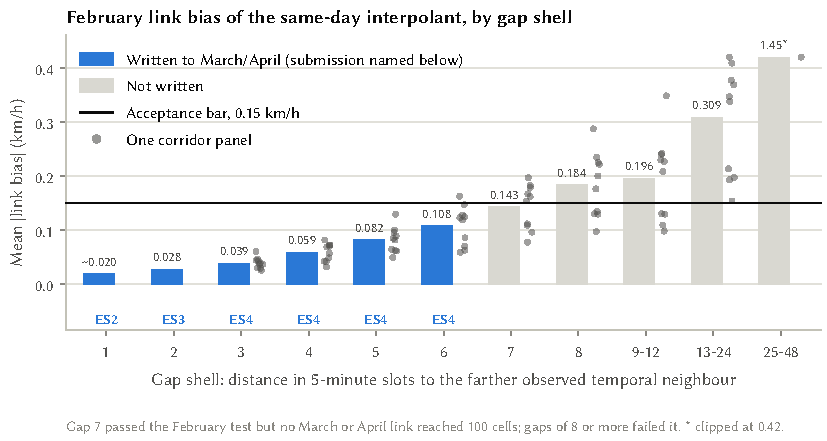
\includegraphics[width=\linewidth]{figures/fig_gap_ladder.pdf}
\caption{The bias test that decided which shells were written. Bars: February mean absolute link bias of the
same-day interpolant, pooled over panels; dots: individual panels. Shells 1--6 passed and were written in three
submissions. Shell 7 passed but no March or April link had the 100 cells the writing rule requires.}\label{fig:gap-ladder}
\end{figure}

\begin{table}[h]
\centering\small
\caption{The gap-shell ladder. February columns are TRAIN proxies; ``changed'' counts March and April speeds;
public $\Delta$ is the Kaggle change of the submission that wrote the shell.}\label{tab:ladder}
\begin{tabular}{@{}l r r r r l@{}}
\toprule
Shell (slots) & Feb.\ link bias & Feb.\ RMSE raw $\rightarrow$ corrected & Speeds changed & Mean $|\Delta v|$ & Public $\Delta$ \\
\midrule
1        & $\approx$0.02 & unchanged & 1,715,267 & 0.962 & +0.00039 (ES2) \\
2        & 0.028 & 2.560 $\rightarrow$ 2.560 & 1,918,477 & 0.960 & +0.00044 (ES3) \\
3        & 0.039 & 2.842 $\rightarrow$ 2.842 & 1,186,051 & \multirow{4}{*}{0.954} & \multirow{4}{*}{+0.00074 (ES4)} \\
4        & 0.059 & 3.085 $\rightarrow$ 3.086 & 671,422 & & \\
5        & 0.082 & 3.423 $\rightarrow$ 3.425 & 319,161 & & \\
6        & 0.108 & 3.562 $\rightarrow$ 3.565 & 15,289 & & \\
7        & 0.143 & 3.646 $\rightarrow$ 3.651 & 0 & --- & not written \\
8        & 0.184 & --- & 0 & --- & failed \\
9--12    & 0.196 & --- & 0 & --- & failed \\
13--24   & 0.309 & --- & 0 & --- & failed \\
25--48   & 1.451 & --- & 0 & --- & failed \\
\bottomrule
\end{tabular}
\end{table}

Across the three submissions the edit changed 5,825,667 speeds by about 0.96 km/h on average (RMS 1.25 km/h,
maximum 6.24 km/h) and added +0.00157 in public. It is a small gain from a simple, label-free statistic, and it is
the only evaluation-month adaptation of speed in the selected files.

\subsection{Results and error analysis}\label{sec:state-error}
\Cref{fig:state-regimes} compares the RS1 residual model with interpolation on February, held out from a fit on
June--November. Speed RMSE falls from 2.75--2.98 to 1.46--1.66 km/h and per-lane flow RMSE from 44.5--47.6 to
30.4--31.1 veh/h, giving a state piece of 0.940--0.945 against 0.899--0.907. The 50\,\% mask costs the model only
0.005 in the piece relative to the 20\,\% mask. \Cref{fig:state-gaps} shows that the advantage holds at every gap
length: the model roughly halves interpolation error from one-slot gaps (1.41 against 2.37 km/h) to gaps of 13--30
slots (1.99 against 3.98 km/h).

\begin{figure}[t]
\centering
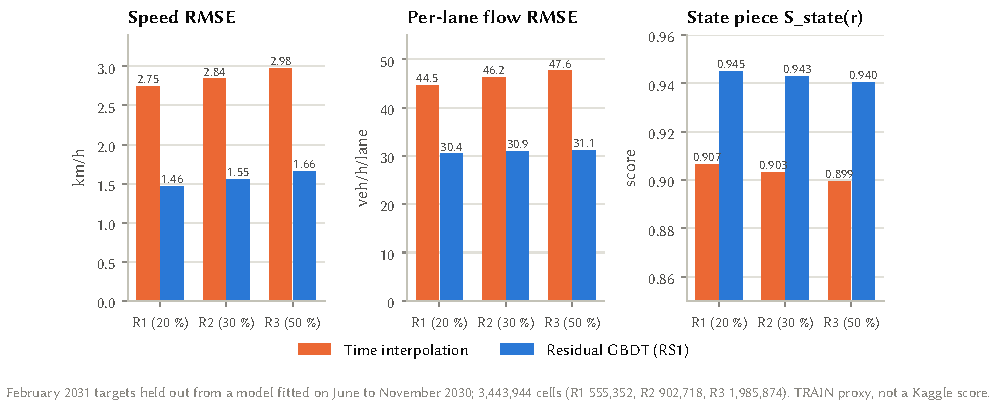
\includegraphics[width=\linewidth]{figures/fig_state_regimes.pdf}
\caption{February state error by masking regime for the residual model and for same-day interpolation.}\label{fig:state-regimes}
\end{figure}

\begin{figure}[t]
\centering
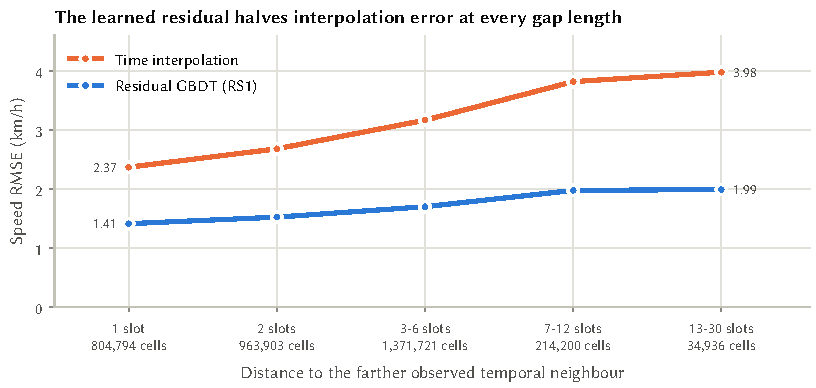
\includegraphics[width=\linewidth]{figures/fig_state_gaps.pdf}
\caption{February speed error by gap length. The residual model's error grows from 1.41 to 1.99 km/h as gaps widen;
interpolation's grows from 2.37 to 3.98 km/h.}\label{fig:state-gaps}
\end{figure}

\paragraph{Where the error is} Error concentrates where a wave passes inside the gap. Among February cells with both
anchors within six slots, 138,195 have anchors that disagree by at least 20 km/h or an interpolant at most
$0.6\,v_f$. There interpolation reaches
10.57 km/h RMSE and the model 4.62 km/h, better on all ten corridors. Same-time neighbours do not substitute for
temporal anchors: on 735,668 cells where both adjacent links are observed, their average scores 6.37 km/h against the
model's 1.44, and switching to the neighbours only when the temporal anchors disagree by 20 km/h still scores
1.60 km/h. The model already combines both sources better than any fixed rule we tried.

\paragraph{What the public board says} Replacing the first residual model by plain interpolation (L0 against U2)
cost 0.00867 in public, and the RS1 model added +0.00974 over the first model (RC2 against RC1). Month-blocked
cross-validation on training months had predicted about +0.021 for the first model over interpolation in the same
state-and-physics block, $0.35\,\Sstate+0.15\,\Sphys$; the public board measured +0.0087. The model transfers to a new month, but less than half
of its cross-validated advantage survived, which is why every later state change was gated on held-out months
and why we treat state proxies as optimistic by a factor of about two.
